\subsection*{(b) }
%
\begin{color}{AAUblue2}
%
Forstå modellen og betydningen af parametrene samt begyndelsesværdierne, ved at udfører numeriske eksperimenter. 
Plot løsningskurven. 
Brug \textsc{opg2-system.py}, og gennemgå koden med henblik på at modificere den. 
Vælg en række andre begyndelsesværdier, parameterne $\alpha$ og $\beta$. Plot også de tre kurver $(t, x_j(t)), j = 1,2,3$ i samme figur.
% 
\end{color}
\\\\
% 
For at få en idé om hvilken betydning parametrene har, er der lavet en række eksperimenter, hvor en enkelt parameter er ændret.
Figur \ref{fig:a1_b35_g0} er udgangspunktet.\\\\
%
\begin{figure}[!ht]
\centering
$
\begin{matrix}
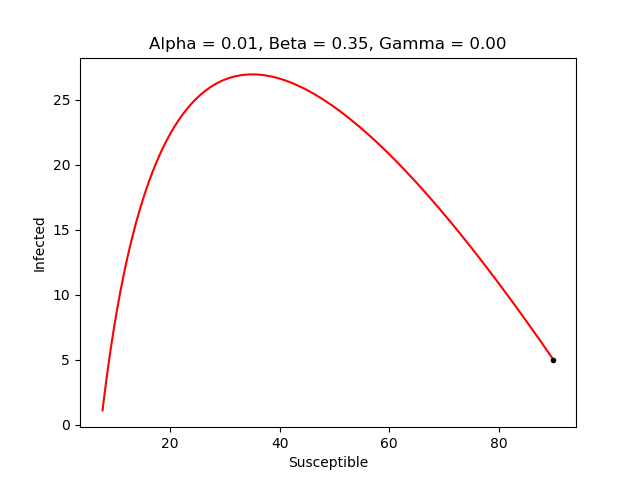
\includegraphics[scale=0.5]{fig/img/a1_b35_g0.png}&
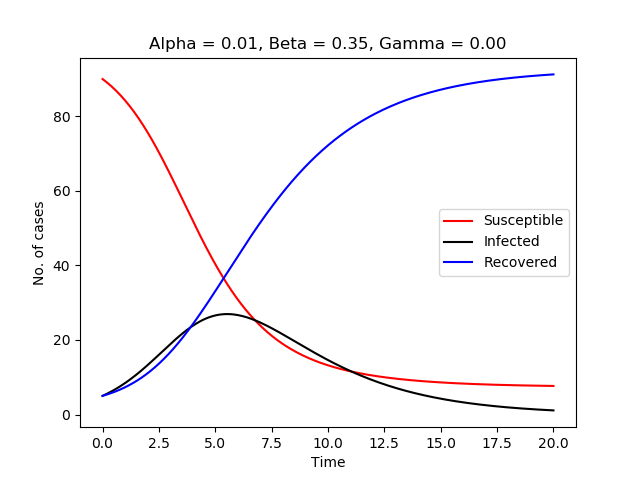
\includegraphics[scale=0.5]{fig/img/t_a1_b35_g0.png}
\end{matrix}
$
\caption{Smitten når $\alpha = 0.01$, $\beta = 0.35$ og $\gamma = 0$.}
\label{fig:a1_b35_g0}
\end{figure}\\\\
%
Først er der gjort en fordobling i $\alpha$, hvor ændringen det har forsaget kan ses på figur \ref{fig:a2_b35_g0}.
%
\begin{figure}[!ht]
\centering
$
\begin{matrix}
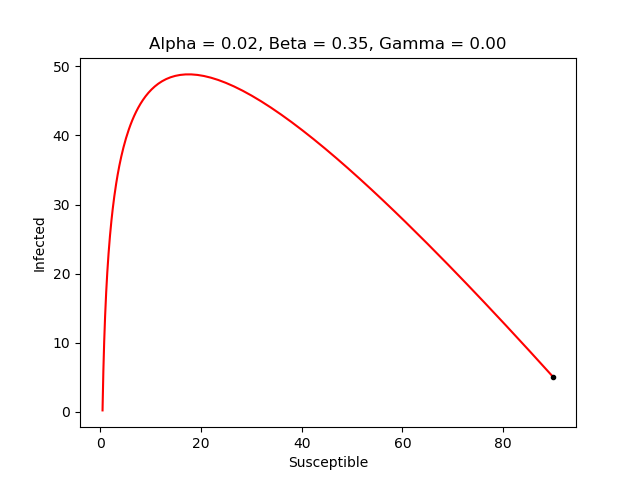
\includegraphics[scale=0.5]{fig/img/a2_b35_g0.png}&
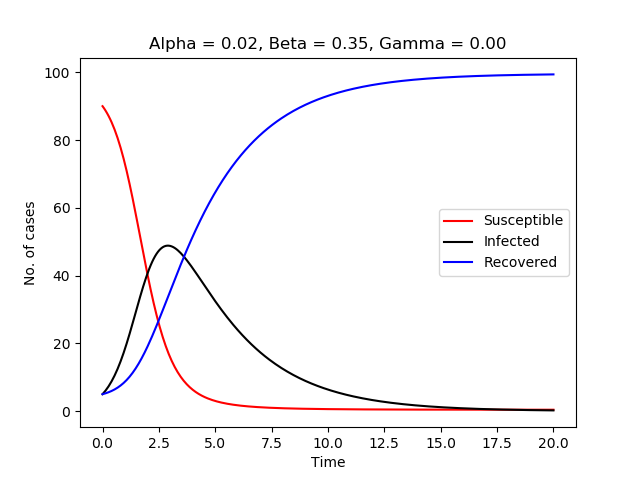
\includegraphics[scale=0.5]{fig/img/t_a2_b35_g0.png}
\end{matrix}
$
\caption{Smitten når $\alpha = 0.02$, $\beta = 0.35$ og $\gamma = 0$.}
\label{fig:a2_b35_g0}
\end{figure}\\\\
%
Her kan det ses, at denne ændring har forsaget smitten til at toppe hurtigere og højere.
Det bør bemærkes, at antallet der kan smittes og immune også er henholdsvis hurtigere faldende og stigende.
Dette virker som en naturlig konklusion, da $\alpha$ beskriver hvor hurtigt smitten kan sprede sig.\\\\
%
Dernæst er der lavet en fordobling af $\beta$, hvor resultatet af dette kan ses på figur \ref{fig:a1_b7_g0}.\\\\
%
\begin{figure}[!ht]
\centering
$
\begin{matrix}
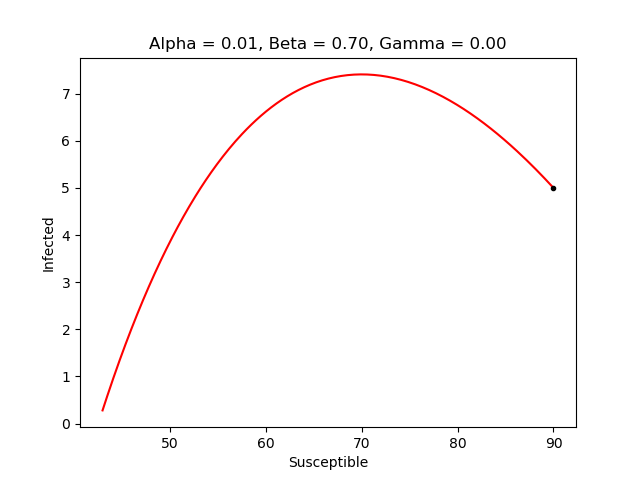
\includegraphics[scale=0.5]{fig/img/a1_b7_g0.png}&
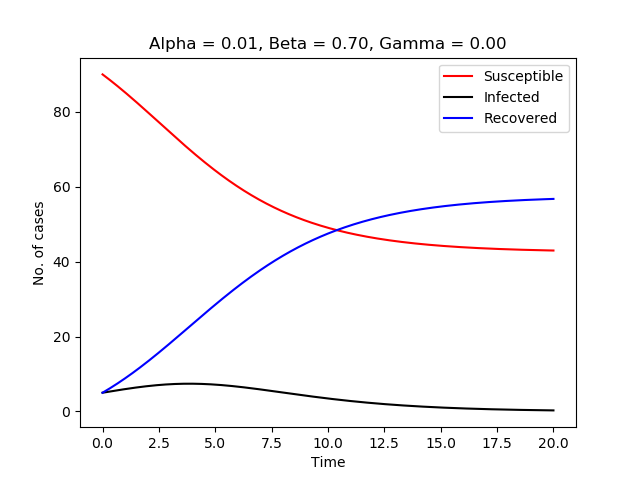
\includegraphics[scale=0.5]{fig/img/t_a1_b7_g0.png}
\end{matrix}
$
\caption{Smitten når $\alpha = 0.01$, $\beta = 0.7$ og $\gamma = 0$.}
\label{fig:a1_b7_g0}
\end{figure}\\\\
%
Her kan det ses, at denne ændring har forsaget smitten til at toppe minimalt hurtigere, men betydeligt lavere.
Dette har ligeledes en effekt på hvor hurtigt folk bliver immune og antallet der kan smittes.
Her ser det ud til at der ikke kommer et punkt, hvor alle er immune, da smitten naturligt uddør inden da.\\\\
%
Nu til effekten af begyndelsesværdierne for antallet af syge og antallet af immune.
På figur \ref{fig:x1_1_x2_95} ses effekten af at det indledende antal af syge er ændret fra $5$ til $1$, lade de $4$, som var syge, være smittelige.
%
\begin{figure}[!ht]
\centering
$
\begin{matrix}
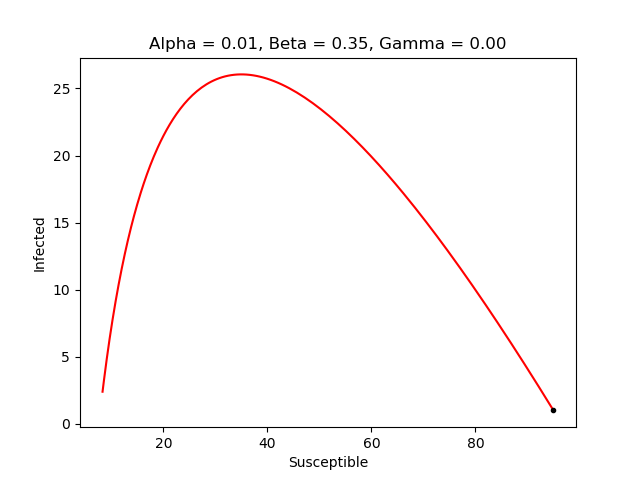
\includegraphics[scale=0.5]{fig/img/x1_1_x2_95.png}&
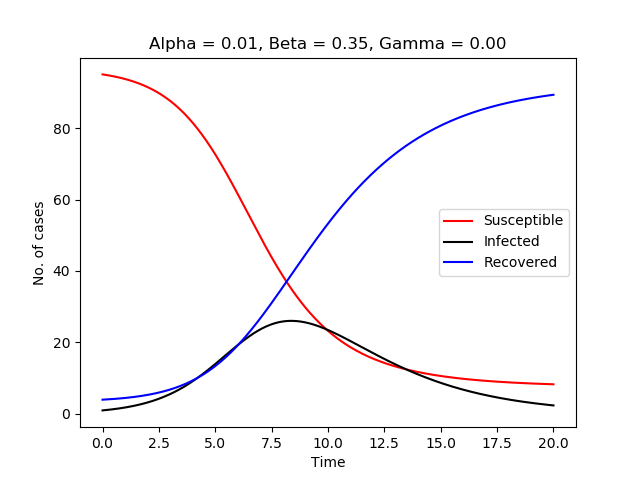
\includegraphics[scale=0.5]{fig/img/t_x1_1_x2_95.png}
\end{matrix}
$
\caption{Smitten når $\alpha = 0.01$, $\beta = 0.7$ og $\gamma = 0.05$.}
\label{fig:x1_1_x2_95}
\end{figure}\\\\
%
Dette lader ikke til at haven anden effekt en at forsænke toppen på smitten.
Ændres det indledende antal af immune til det dobbelte, kan effekten af dette ses på figur \ref{fig:x1_5_x2_85}.
%
\begin{figure}[!ht]
\centering
$
\begin{matrix}
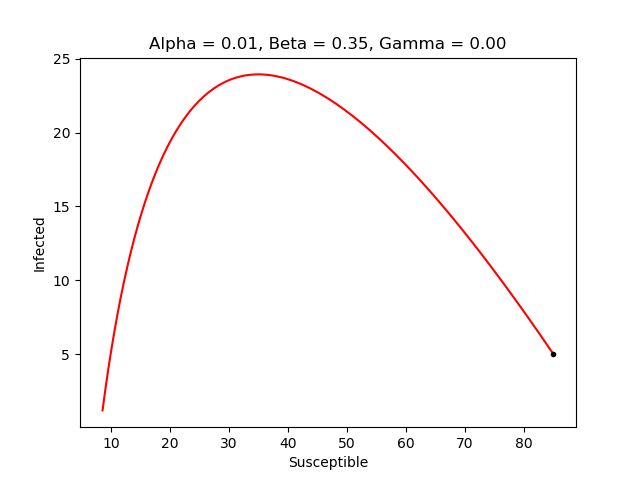
\includegraphics[scale=0.5]{fig/img/x1_5_x2_85.png}&
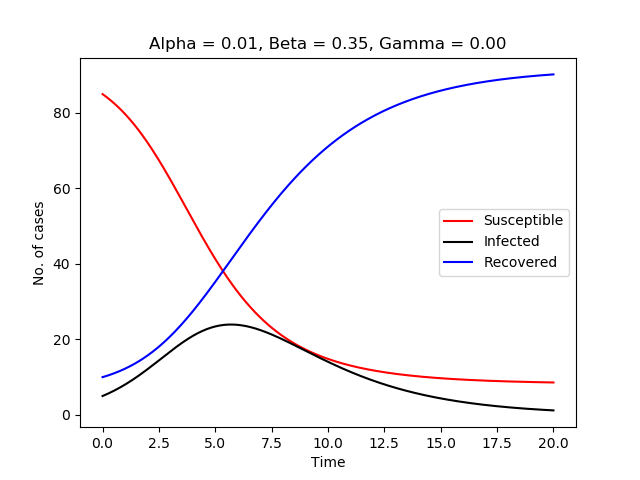
\includegraphics[scale=0.5]{fig/img/t_x1_5_x2_85.png}
\end{matrix}
$
\caption{Smitten når $\alpha = 0.01$, $\beta = 0.7$ og $\gamma = 0.05$.}
\label{fig:x1_5_x2_85}
\end{figure}\\\\
%
Dette har ikke den store betydning, men smittens top er dog faldet lidt, og der er i dette tilfælde ikke noget punkt, hvor der er flere syge end immune eller smittelige.